\chapter{C's Memory Model}
\label{ch:mem}

\newcommand{\lecnum}{20}
%\newcommand{\lectitle}{C's Memory Model}
\newcommand{\lecturer}{Frank Pfenning, Rob Simmons}

\chapterTAGS{aliasing, c-array, c-memory, memory-model, safety, undefined-behavior}
\maketitle

\begin{preamble}
  \noindent
  In this lecture, we'll talk about the differences between the memory
  model we developed in C0, with local and allocated sections, and the
  memory model that C uses. Much of the model will stay the same, but
  we'll go more in depth and learn some new terms.
\end{preamble}


\section{The C0 and C Memory Model}
\label{sec:mem:memory_models}
\TAGS{memory-model}

When we talk about memory in C0, C1, and C, that memory is always in one
of three places:
\begin{itemize}
\item%
  \emph{Local variables} (including the arguments to functions) are stored in
  memory. In both C0 and C, this memory is reserved automatically when we
  declare a new local variable, though in C the contents of that local memory
  aren't initialized. The local memory gets reclaimed as soon as the local
  variable goes out of scope.
\item%
  \emph{Allocated memory} was reserved with \lstinline'alloc' and
  \lstinline'alloc_array'. We always accessed this memory by referring to its
  address (the address stored in a non-\lstinline'NULL' pointer or the address
  of an array). When we reserved allocated memory in C0, this memory was
  initialized to default values for us. In C, \lstinline'xmalloc' does not
  initialize memory.
\item%
  In C1, we said that the compiled code for functions was stored in
  \emph{read-only memory}, and we could get pointers into that read-only
  memory by taking the address of a function: \lstinline'&f'.  Many more
  things in C are stored in read-only memory, like string literals.
\end{itemize}

In this class, we think about \emph{all} of this data residing in
memory.\footnote{Later classes will complicate this picture by talking about
  things like \emph{registers} that you don't need to know about in 15-122.} In
this picture, memory is comprised of an enormous array of bytes, where each
index in the array of bytes is an address. The lowest address is 0, and the
highest address on most modern, 64-bit processors is $2^{64} - 1 =
\texttt{0xFFFFFFFFFFFFFFFF}$.  This is an almost inconceivably large array of
bytes, far larger than the physical RAM installed in \emph{any} computer, but
the operating system plays tricks to allow processors to pretend like they
have access to this enormous array. One way this is done is by only giving
programs access to individual \emph{segments} of this array. Modern hardware
prevents individual running programs from accessing memory outside their
allocated segments. (This is a good thing: it means that, no matter how much
you mess up while programming in C, it's going to be difficult for you to
interfere with other running programs like your text editor or virus scanner.)

The memory used for the local variables of a function is allocated and
de-allocated according to a stack discipline, so we call this portion of
memory the \emph{stack}. Memory that we explicitly allocate is reserved in
what we call the \emph{heap}, though it has no relationship to the heap data
structure. Read-only memory is also called the \emph{text} region. Therefore,
the big picture of memory looks like this:
\begin{lstlisting}[language=c]
0xFFFFFFFFFFFFFFFF        |
                          | OS AREA
                          | ============
                          | System stack   (local variables)
                          | ============
                          | unused
                          | ============
                          | System heap    (allocated memory)
                          | ============
                          | .text          (read only memory)
                          | ============
                          | OS AREA
0x0000000000000000        |
\end{lstlisting}

One consequence of this memory layout is that the stack grows towards
the heap, and the heap usually grows towards the stack.  Programs
cannot access addresses (indices in this enormous array) that belong
to the operating system.  If they try, programs get an ``exception''
like a segmentation fault.  C0 takes great care to ensure that it
never gives you any pointers to uninitialized or random or garbage
data in memory, \emph{except}, of course, the \lstinline'NULL' pointer.
\lstinline'NULL' is a special pointer to the memory address 0, which
belongs to the operating system. The address 0 will usually not be a
part of one of the memory segments you are allowed to read from or
write to, so accessing the \lstinline'NULL' pointer causes you to read or
write outside of your segment: a \emph{segmentation fault}, or
segfault.


\section{Arrays and Pointer Arithmetic}
\label{sec:mem:pointer_arith}
\TAGS{aliasing, c-array, c-memory, memory-model}

When compared to C0, the most shocking difference is that C does not
distinguish arrays from pointers. We allocate enough space for a
single integer by writing \lstinline'sizeof(int)', and we allocate enough
space for an array of 5 integers by just multiplying the size of a
single integer by 5.
\begin{lstlisting}[language=c]
int *A = xmalloc(sizeof(int) * 5);
for (size_t i = 0; i < 5; i++) A[i] = i*i*i*i;
\end{lstlisting}

Assuming 4-byte integers, this 5 element array is treated by C as no
more and no less than a single 20 byte memory segment that we are
allowed to use. If the call to \lstinline'malloc' returned the memory
address \lstinline'0xCA0', then after the \lstinline'for' loop is
done, the four bytes of memory addressed by \lstinline'0xCA8' to
\lstinline'0xCAB' will together represent the integer 16, the contents
of the third index of the array, \lstinline'A[2]', and so on:
\begin{center}
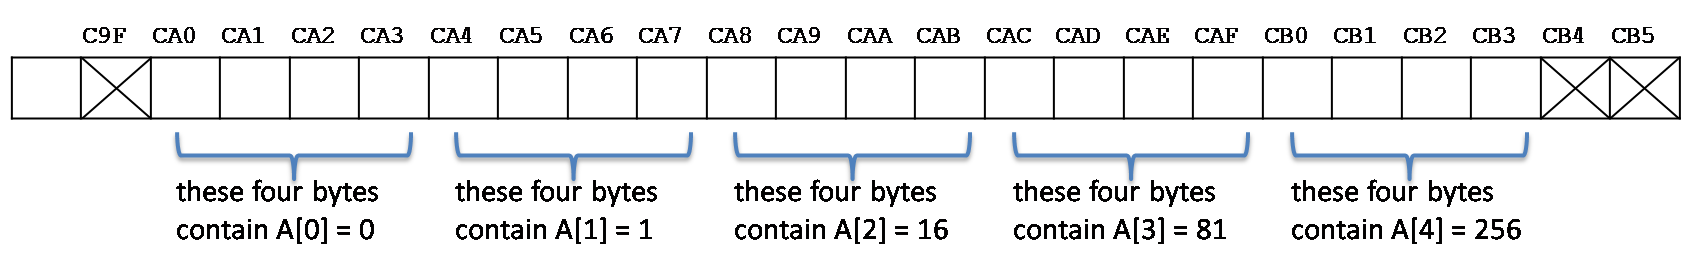
\includegraphics[width=0.95\textwidth]{img/allocation.png}
\end{center}

One consequence of this conflation of pointers and arrays is that
writing \lstinline'*A' and writing \lstinline'A[0]' necessarily means
the same thing.  We can also add an integer to a pointer, but this
modifies the pointer not in terms of bytes but in terms of array
elements. This allows us to get pointers into arrays!
\begin{lstlisting}[language=c]
int *x = A + 3;
*x += 5;
\end{lstlisting}
In the example above, then after running these two lines, the local
variable \lstinline'x' will contain the pointer \lstinline'0xCAC', and
the assignment will cause both \lstinline'*x' and \lstinline'A[3]' to
evaluate to 86 instead of 81. This is a form of aliasing that was
impossible in C0, but it is relatively common in C. But because only
the pointer \lstinline'0xCA0' in the example above was returned from
\lstinline'xmalloc', only that pointer should be freed: it would be a
memory error to free the pointer \lstinline'0xCAC' stored in
\lstinline'x'.

When we allocate very large arrays, we may want them allocated with
default values, the way we did in C0. The C standard library provides a
function, \lstinline'calloc', to do just that, and our \lstinline'xalloc.h'
library has a non-\lstinline'NULL'-returning \lstinline'xcalloc' version of
\lstinline'calloc' that you should use. With \lstinline'xcalloc', we can allocate
an array of seven elements, all of which are initialized to 0, like this:
\begin{lstlisting}[language=c]
int *B = xcalloc(7, sizeof(int));
for (size_t i = 1; i < 7; i++) A[i] = A[i-1]*2 + 3;
\end{lstlisting}
The only differences between \lstinline'xmalloc' and \lstinline'xcalloc' is that
the latter initializes the memory to be all zeroes and takes two
arguments. The \lstinline'xcalloc' function takes two sizes $n$
and $m$ and allocates $n\times m$ bytes. We
think of \lstinline'xmalloc' as being like C0's \lstinline'alloc' and we think
of \lstinline'xcalloc' as being like C0's \lstinline'alloc_array', but in C you
can allocate arrays and pointers with either \lstinline'xmalloc' or
\lstinline'xcalloc'.


\section{Undefined Behavior}
\label{sec:mem:undefined_behavior}
\TAGS{c-array, safety, undefined-behavior}

We have described the following as memory errors:
\begin{itemize}
\item%
  Reading uninitialized memory (on the stack or on the heap).
\item%
  Dereferencing memory outside of a valid allocated segment (which includes
  \lstinline'NULL' pointer dereference, array out of bounds errors), or trying
  to read or write to an \lstinline'int' when you've only allocated enough
  size for a \lstinline'char'.
\item%
  Writing to memory that is in a read-only segment like \lstinline'.text'.
\item%
  Using a memory allocation that has been freed, double-freeing a pointer, or
  freeing any pointer that wasn't returned from \lstinline'xmalloc' or
  \lstinline'xcalloc'.
\end{itemize}
In C0, memory errors would always predictably and consistently cause
the program to stop executing. In C, this is \emph{definitely not the case}.

Array accesses are not checked at all, and out-of-bounds memory
references (whose result is formally undefined) may lead to
unpredictable results. The program might stop with an error, or keep
going, but after undefined behavior occurs it is difficult, if not
impossible, to predict a program's behavior. For example, the code
fragment
\begin{lstlisting}[language=c, numbers=left]
int main() {
  int* A = xmalloc(sizeof(int));
  A[0] = 0;         /* ok - A[0] is like *A */
  A[1] = 1;         /* error - not allocated */
  A[317] = 29;      /* error - not allocated */
  A[-1] = 32;       /* error - not allocated(!) */
  printf("A[-1] = %d\n", A[-1]);
  return 0;
}
\end{lstlisting}
will not raise any compile time error or even warnings, even under the
strictest settings.  Here, the call to \lstinline'xmalloc' allocates enough
space for a single integer in memory.  In this class, we are using
\lstinline'gcc' with all our standard flags:

\begin{lstlisting}[language={[coin]C}]
% gcc -Wall -Wextra -Wshadow -Werror -std=c99 -pedantic -g
\end{lstlisting}
The code
above executes ok, and in fact prints \lstinline'32', despite four blatant
errors in the code.

To discover whether such errors may have occurred
at runtime, we can use the \lstinline'valgrind' tool.
\begin{lstlisting}[language={[coin]C}]
% valgrind ./a.out
...
==nnnn== ERROR SUMMARY: 4 errors from 4 contexts (suppressed: 0 from 0)
\end{lstlisting}
which produces useful error messages (elided above) and indeed,
flags errors in code that didn't appear to have any errors when we ran
it without \lstinline'valgrind'.

% \lstinline'valgrind' slows down execution, but if at all feasible you
% should use it to test all your C code to uncover memory
% problems.  For best error messages, you should pass the \lstinline'-g'
% flag to \lstinline'gcc' which preserves some correlation between
% binary and source code.

You can also guard memory accesses with appropriate \lstinline'assert'
statements that abort the program when attempting out-of-bounds accesses.

There's an old joke that
whenever you encounter undefined behavior, your computer could decide
to play \emph{Happy Birthday} or it could catch on fire. This is less
of a joke considering recent events:
\begin{itemize}
\item%
  In 2010, Alex Halderman's team at the University of Michigan successfully
  hacked into Washington D.C.'s prototype online voting system, and caused its
  web page to play the University of Michigan fight song, ``The
  Victors.''\footnote{Scott Wolchok, Eric Wustrow, Dawn Isabel, and J. Alex
    Halderman. \emph{Attacking the Washington, D.C.~Internet Voting System}.
    Proceedings of the 16th Conference on Financial Cryptography and Data
    Security, February 2012.}
\item%
  The Stuxnet worm caused centrifuges, such as those used for uranium
  enrichment in Iran, to malfunction, physically damaging the
  devices.\footnote{Holger Stark. \emph{Stuxnet Virus Opens New Era of Cyber
      War}. Spiegel Online, August 8, 2011.}
\end{itemize}
Not quite playing \emph{Happy Birthday} and catching on fire, but close
enough.

\section{Address-of}
\label{sec:mem:address_of}
\TAGS{c-memory}

In our C0 and C memory model, almost \emph{everything} has an
address. If \lstinline'e' is an expression (like \lstinline'x',
\lstinline'A[12]', \lstinline'*x', \lstinline'A.fld', or
\lstinline'A->fld') that describes a memory location which we can read
from and potentially write to, then that memory location exists in
memory as some number of bytes with an address.  Writing
\lstinline'&e' then gives us a \emph{pointer} to that memory
location. In C0, if we have a struct containing a string and an
integer, it's not possible to get a pointer to \emph{just} the
integer. This is possible in C:
\begin{lstlisting}[language=c]
struct wcount {
  char *word;
  int count;
};

void increment(int *p) {
  REQUIRES(p != NULL);
  *p = *p + 1;
}

void increment_count(struct wcount *wc) {
  REQUIRES(wc != NULL);
  increment(&(wc->count));
}
\end{lstlisting}
Because the type of \lstinline'wc->count' is \lstinline'int', the expression
\lstinline'&(wc->count)' is a pointer to an \lstinline'int'.  Calling
\lstinline'increment_count(B)' on a non-null struct will cause the
\lstinline'count' field of the struct to be incremented by the
\lstinline'increment' function, which is passed a pointer to the second
field of the struct.

Because of the address-of operation, we never have to actually use
pointer arithmetic if we don't want to.  For example,
\lstinline'&A[3]' is equivalent to \lstinline'A + 3', and much more readable.


\section{Stack Allocation}
\label{sec:stack_allocation}
\TAGS{aliasing, c-array, c-memory, safety}

%\enlargethispage{2ex}

In C, we can also allocate data on the \emph{system stack} (which is
different from the explicit stack data structure you have studied).
Each function allocates memory in its so-called \emph{stack frame} for
local variables.  We can obtain a pointer to this memory using the
address-of operator.  For example:
\begin{lstlisting}[language=c]
int main() {
  int a1 = 1;
  int a2 = 2;
  increment(&a1);
  increment(&a2);
  ...
}
\end{lstlisting}
Note that there is no call to \lstinline'xmalloc' or \lstinline'xcalloc' which
allocate spaces on the system heap (again, this is different from the
heap data structure we used for priority queues).

We can only free memory allocated with \lstinline'xmalloc'
or \lstinline'xcalloc', but not memory that is on the system stack.
Such memory will automatically be freed when the function whose
frame it belongs to returns.  This has two important consequences.
The first is that the following is a bug, because \lstinline'free'
will try to free the memory holding \lstinline'a1', which is
not on the heap:
\begin{lstlisting}[language=c]
int main() {
  int a1 = 1;
  int a2 = 2;
  free(&a1);  // BUG: trying to free a local variable
  ...
}
\end{lstlisting}
%Instead, we must call \lstinline'stack_free(S, NULL)'.
The second consequence is pointers to data stored on the system stack
do not survive the function's return.  For example, the following is a
bug:
\begin{lstlisting}[language=c]
int *f_ohno() {
  int a = 1;  // BUG: a is deallocated when f_ohno() returns
  return &a;
}
\end{lstlisting}
(recent versions of \lstinline'gcc' recognize that this makes little
sense and issue a compilation error).  A correct implementation
requires us to allocate on the system heap, using a call to
\lstinline'malloc' or \lstinline'calloc' (or one of the library
functions which calls them in turn).
\begin{lstlisting}[language=c]
int *f() {
  int* x = xmalloc(sizeof(int));
  *x = 1;
  return x;
}
\end{lstlisting}

C offers a special syntax to allocate \emph{arrays} on the stack.  The
following \lstinline'main' declares an array \lstinline'A' with 5
elements, initializes it, calls the function \lstinline'sum' which
adds up its elements, and prints the result.
\begin{lstlisting}[language=c]
int sum(int* A, int n) {
  int res = 0;
  for (int i = 0; i < n; i++)
    res += A[i];
  return res;
}

void main() {
  int A[5];
  for (int i=0; i < 5; i++)
    A[i] = i;
  printf("%d\n", sum(A, 5));
}
\end{lstlisting}
C even provides syntax to initialize a literal array, i.e., an array
whose length and contents are fixed values.  The above
\lstinline'main' function can indeed be rewritten as follows:
\begin{lstlisting}[language=c]
void main() {
  int A[] = {0, 1, 2, 3, 4};
  printf("%d\n", sum(A, 5));
}
\end{lstlisting}
Note that it's not even necessary to specify the length of
\lstinline'A': the compiler figures it out.


\medskip
When stack allocation is possible, it can be a real benefit,
because it saves you from having to remember to free memory explicitly.
However, if the data structure we allocate needs to
survive past the end of the current function you \emph{must} allocate
it on the heap.
